\begin{name}
	{\tenchude}
	{\tendethi}
	{\tentruong}
	{\thoigian}
\end{name}
\TN
\Opensolutionfile{ans}[ans/ans\currfilebase]
%%%==============Cau_EX1==============%%%
\begin{ex}%[2D1N2-2]%[Lớp 12 - Đề thi GK1 - THPT Ba Điềm - TPHCM]%[Hoàng Anh Tuấn]
	Cho hàm số $y=f(x)$ có bảng biến thiên như sau:
	\begin{center}
		
\begin{tikzpicture}
			\tkzTabInit[nocadre=false,espcl=2.5,lgt=1.5,deltacl=0.6]
			{$x$/0.7,$f'(x)$/0.7,$f(x)$/2}
			{$-\infty$,$0$,$3$,$+\infty$}
			\tkzTabLine{,+,0,-,0,+,}
			\tkzTabVar{-/$-\infty$,+/$2$,-/$-4$,+/$+\infty$}
		\end{tikzpicture}
	\end{center}
	Giá trị cực tiểu của hàm số đã cho bằng
	\choice
	{$3$}
	{\True $4$}
	{$2$}
	{$0$}
	\loigiai{
		Dựa vào bảng biến thiên, ta thấy giá trị cực tiểu của hàm số là $-4$.
	}
\end{ex}

%%%==============HetCau_EX1==============%%%

%%%==============Cau_EX2==============%%%
\begin{ex}%[2D1N4-1]%[Lớp 12 - Đề thi GK1 - THPT Ba Điềm - TPHCM]%[Hoàng Anh Tuấn]
Cho hàm số $y=f(x)$ có $\lim\limits_{x\to+\infty}f(x)=1$ và  $\lim\limits_{x\to-\infty}f(x)=-1$. Khẳng định nào sau đây là khẳng định đúng?
	\choice
	{Đồ thị hàm số đã cho có đúng một tiệm cận ngang}
	{Đồ thị hàm số đã cho không có tiệm cận ngang}
	{\True Đồ thị hàm số đã cho có hai tiệm cận ngang là các đường thẳng $y=1$ và $y=-1$}
	{Đồ thị hàm số đã cho có hai tiệm cận ngang là các đường thẳng $x=1$ và $x=-1$}
	\loigiai{
	Theo định nghĩa đường tiệm cận ngang ta có
	\begin{itemize}
		\item $\lim\limits_{x\to+\infty}f(x)=1\Rightarrow y=1$ là một đường tiệm cận ngang.
		\item $\lim\limits_{x\to-\infty}f(x)=-1\Rightarrow y=-1$ là một đường tiệm cận ngang.
	\end{itemize}
	}
\end{ex}

%%%==============HetCau_EX2==============%%%

%%%==============Cau_EX3==============%%%
\begin{ex}%[2D1H3-1]%[Lớp 12 - Đề thi GK1 - THPT Ba Điềm - TPHCM]%[Hoàng Anh Tuấn]
Tìm giá trị lớn nhất $M$ của hàm số $y=\dfrac{3x-1}{x-3}$ trên đoạn $[0;2]$.
	\choice
	{\True $M=\dfrac{1}{3}$}
	{$M=-\dfrac{1}{3}$}
	{$M=5$}
	{$M=5$}
	\loigiai{
	Ta có $y=\dfrac{3x-1}{x-3}\Rightarrow y'=\dfrac{-8}{(x-3)^2}<0, \forall x\neq 3$.\\
	 Suy ra hàm số nghịch biến trên đoạn $[0;2]$. Vậy $\max\limits_{[0;2]}y=y(0)=\dfrac{1}{3}.$
	}
\end{ex}

%%%==============HetCau_EX3==============%%%

%%%==============Cau_EX4==============%%%
\begin{ex}%[2D1H3-1]%[Lớp 12 - Đề thi GK1 - THPT Ba Điềm - TPHCM]%[Hoàng Anh Tuấn]
	Cho hàm số $y=f(x)$ xác định trên đoạn $[-\sqrt{3};\sqrt{5}]$ và có bảng biến thiên như hình vẽ. 
	\begin{center}
		\begin{tikzpicture}
		\tkzTabInit[nocadre=false,espcl=2.7,lgt=1.6,deltacl=0.8]
		{$x$/0.7,$f'(x)$/0.7,$f(x)$/2}
		{$-\sqrt{3}$,$-1$,$1$,$\sqrt{5}$}
		\tkzTabLine{,+,0,-,0,+,}
		\tkzTabVar{-/$0$,+/$2$,-/$-2$,+/$2\sqrt{5}$}
	%	\draw (1.25,-4) rectangle (3,1);
		\draw[opacity=0.5,pattern=north west lines] (1.6,-3.5) rectangle (2.4,-0.7) ;
	%	\node[above,fill=white]  at (2.5,-3.5) {$0$};
		\draw[opacity=0.4,pattern=north west lines] (10.5,-3.5) rectangle (11.3,-0.7) ;
	%	\node[above,fill=white] at (10.5,-2.25) {$2\sqrt{5}$};
	\end{tikzpicture}
	\end{center}
	Khẳng định nào sau đây là đúng?
	\choice
	{$\min\limits_{[-\sqrt{3};\sqrt{5}]}y=0$ }
	{\True $\max\limits_{[-\sqrt{3};\sqrt{5}]}y=2\sqrt{5}$ }
	{$\min\limits_{[-\sqrt{3};\sqrt{5}]}y=1$ }
	{$\max\limits_{[-\sqrt{3};\sqrt{5}]}y=2$ }
	\loigiai{
	Từ bảng biến thiên, ta thấy hàm số đạt giá trị nhỏ nhất bằng $-2$ tại $x = 1$ và đạt giá trị lớn nhất bằng $2\sqrt{5}$ tại $x=\sqrt{5}$.
	}
\end{ex}

%%%==============HetCau_EX4==============%%%


%%%==============Cau_EX5==============%%%
\begin{ex}%[2D1H4-1]%[Lớp 12 - Đề thi GK1 - THPT Ba Điềm - TPHCM]%[Hoàng Anh Tuấn]
Cho hàm số $y=\dfrac{x^2+2x-1}{2x-1}$ có đồ thị $(C)$. Tiệm cận xiên của đồ thị hàm số là:
	\choice
	{$y=2x-1$ }
	{$y=\dfrac{1}{2}x+\dfrac{5}{2}$ }
	{\True$y=\dfrac{1}{2}x+\dfrac{5}{4}$ }
	{$x=1$ }
	\loigiai{
		Ta thấy hàm số có dạng phân thức, bậc tử lớn hơn bậc mẫu 1 đơn vị, nên đồ thị hàm số có tiệm cận xiên. Để tìm tiệm cận xiên, ta thực hiện phép chia đa thức:
		$$x^2+2x-1=\left(\dfrac{1}{2}x+\dfrac{5}{4}\right)(2x-1)-\dfrac{1}{4}.$$
		Do đó, ta có  $y=\dfrac{x^2+2x-1}{2x-1}=\dfrac{1}{2}x+\dfrac{5}{4}-\dfrac{1}{4(2x-1)}$. Mà khi $x\to\pm\infty$ thì $-\dfrac{1}{4(2x-1)}\to 0$. \\
		Do đó, tiệm cận xiên của của đồ thị hàm số là $y=\dfrac{1}{2}x+\dfrac{5}{4}$.
	}
\end{ex}

%%%==============HetCau_EX5==============%%%


%%%==============Cau_EX6==============%%%
\begin{ex}%[2D1H1-1]%[Lớp 12 - Đề thi GK1 - THPT Ba Điềm - TPHCM]%[Hoàng Anh Tuấn]
	Cho hàm số $y=x^3-2x^2+x+1$. Mệnh đề nào đưới đây đúng?
	\choice
	{\True Hàm số nghịch biến trên $\left(\dfrac{1}{3};1\right)$ }
	{Hàm số đồng biến trên $\left(\dfrac{1}{3};1\right)$ }
	{Hàm số nghịch biến trên $\left(-\infty;\dfrac{1}{3}\right)$ }
	{Hàm số nghịch biến trên $\left(1;+\infty\right)$}
	\loigiai{
	Ta có: $y=x^3-2x^2+x+1\Rightarrow y'=3x^2-4x+1$. \\
	$y'=0\Leftrightarrow\hoac{x=1\\x=\dfrac{1}{3}}$. Ta có bảng biến thiên sau:
		\begin{center}
		
\begin{tikzpicture}
			\tkzTabInit[nocadre=false,espcl=2.5,lgt=1.5,deltacl=0.6]
			{$x$/0.7,$y'$/0.7,$y$/2.1}
			{$-\infty$,$\frac{1}{3}$,$1$,$+\infty$}
			\tkzTabLine{,+,0,-,0,+,}
			\tkzTabVar{-/$-\infty$,+/$\frac{31}{27}$,-/$1$,+/$+\infty$}
		\end{tikzpicture}
	\end{center}
	Từ bảng biến thiên, ta thấy hàm số nghịch biến trên khoảng $\left(\dfrac{1}{3};1\right)$.
	}
\end{ex}

%%%==============HetCau_EX6==============%%%


%%%==============Cau_EX7==============%%%
\begin{ex}%[2D1H2-1]%[Lớp 12 - Đề thi GK1 - THPT Ba Điềm - TPHCM]%[Hoàng Anh Tuấn]
Hàm số nào sau đây không có cực trị?
	\choice
	{$y=\dfrac{x^2+1}{x}$ }
	{\True $y=\dfrac{2x-2}{x+1}$ }
	{$y=x^2-2x+1$ }
	{$y=-x^3+x+1$}
	\loigiai{
	Ta thấy hàm số $y=\dfrac{2x-2}{x+1}$ có đạo hàm $y'=\dfrac{4}{(x+1)^2}>0,\forall x\neq -1$.\\
	 Do đó hàm số không có cực trị.
	}
\end{ex}

%%%==============HetCau_EX7==============%%%

%%%==============Cau_EX8==============%%%
\begin{ex}%[2D1N1-2]%[Lớp 12 - Đề thi GK1 - THPT Ba Điềm - TPHCM]%[Hoàng Anh Tuấn]
	Cho hàm số $f(x)$ có bảng biến thiên như sau:
		\begin{center}
		
\begin{tikzpicture}
			\tkzTabInit[nocadre=false,espcl=2.5,lgt=1.5,deltacl=0.6]
			{$x$/0.7,$f'(x)$/0.7,$f(x)$/2}
			{$-\infty$,$-3$,$0$,$3$,$+\infty$}
			\tkzTabLine{,-,0,+,0,-,0,+}
			\tkzTabVar{+/$-\infty$,-/$-1$,+/$1$,-/$-1$,+/$\infty$}
		\end{tikzpicture}
	\end{center}
	Hàm số đã cho đồng biến trên khoảng nào sau đây?
	\choice
	{\True $(-3;0)$ }
	{$(-\infty;-3)$}
	{$(0;3)$ }
	{$(-3;3)$}
	\loigiai{
		Từ bảng biến thiên, ta thấy hàm số đồng biến trên khoảng $(-3;0)$.
	}
\end{ex}

%%%==============HetCau_EX8==============%%%

%%%==============Cau_EX9==============%%%
\begin{ex}%[2D1H5-3]%[Lớp 12 - Đề thi GK1 - THPT Ba Điềm - TPHCM]%[Hoàng Anh Tuấn]
	Cho hàm số bậc ba $f(x)$ có đồ thị là đường cong như hình bên. Có bao nhiêu giá trị nguyên của tham số $m$ để phương trình $f(x)=m$ có 3 nghiệm thực phân biệt?
	\begin{center}
			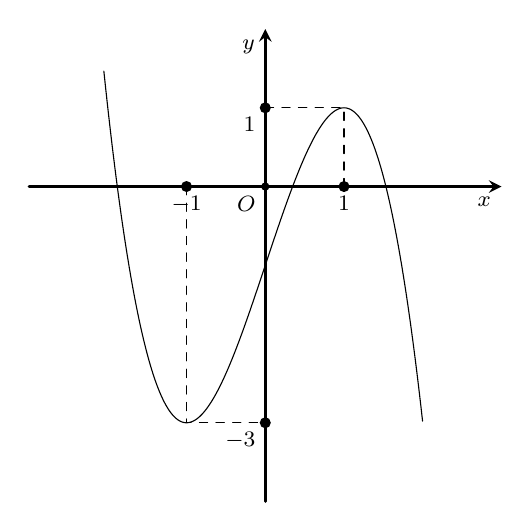
\begin{tikzpicture}[line join = round, line cap=round,>=stealth,font=\footnotesize,scale=1,samples=200]
			
			\def \xtrai{-3} \def\xphai{3}
			\draw[->,line width=1pt] (\xtrai,0)--(\xphai,0) coordinate (x) node[below left]{$x$};	
			\def \yduoi{-4} \def\ytren{2}
			
			\draw[->,line width=1pt] (0,\yduoi)--(0,\ytren)coordinate (y) node[below left]{$y$};			
			
			draw[opacity=0.1] (\xtrai,\yduoi) grid (\xphai,\ytren);
			\fill (0,0) coordinate (O) circle(1.5pt) node[below left]{$O$};
			\draw  plot[domain=-2.05:2] (\x,{-1*(\x)^3+3*(\x)-1})
			;
			\draw[dashed] 
			(-1,0)--(-1,-3) -- (0,-3)
			(0,1)--(1,1) -- (1,0)
		
			;
			\foreach	\x	in	{-1,1}
			\fill (\x,0) circle(2pt) node[below]{$\x$}
			;
			\foreach	\y	in	{-3,1}
			\fill (0,\y) circle(2pt) node[below left]{$\y$}
			;
		\end{tikzpicture}
	\end{center}
	\choice 
	{$5$}
	{$4$}
	{$2$}
	{\True $3$}
	\loigiai{
		Số nghiệm của phương trình $f(x)=m$ bằng số giao điểm của  đồ thị hàm số và đường thẳng $y=m$.
			\begin{center}
			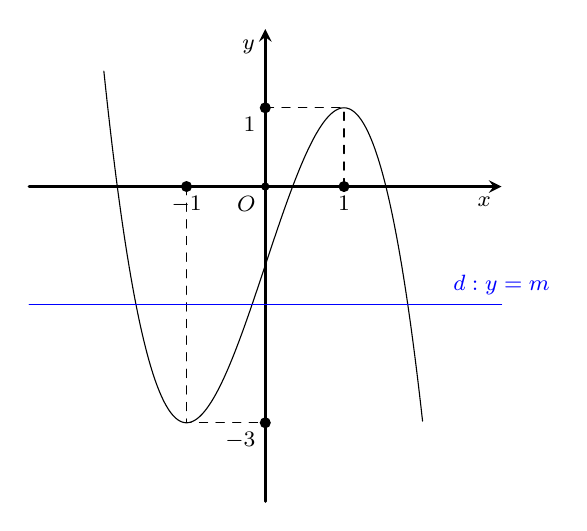
\begin{tikzpicture}[line join = round, line cap=round,>=stealth,font=\footnotesize,scale=1,samples=200]
				
				\def \xtrai{-3} \def\xphai{3}
				\draw[->,line width=1pt] (\xtrai,0)--(\xphai,0) coordinate (x) node[below left]{$x$};	
				\def \yduoi{-4} \def\ytren{2}
				
				\draw[->,line width=1pt] (0,\yduoi)--(0,\ytren)coordinate (y) node[below left]{$y$};			
				
				draw[opacity=0.1] (\xtrai,\yduoi) grid (\xphai,\ytren);
				\fill (0,0) coordinate (O) circle(1.5pt) node[below left]{$O$};
				\draw  plot[domain=-2.05:2] (\x,{-1*(\x)^3+3*(\x)-1})
				;
				\draw[dashed] 
				(-1,0)--(-1,-3) -- (0,-3)
				(0,1)--(1,1) -- (1,0)
				
				;
				\draw[blue] (-3,-1.5)--(3,-1.5) node[above]{$d: y=m$};
				\foreach	\x	in	{-1,1}
				\fill (\x,0) circle(2pt) node[below]{$\x$}
				;
				\foreach	\y	in	{-3,1}
				\fill (0,\y) circle(2pt) node[below left]{$\y$}
				;
			\end{tikzpicture}
		\end{center}
		Dựa vào hình vẽ, ta thấy phương trình $f(x)=m$ có ba nghiệm thực phân biệt khi đường thẳng $d:y=m$ cắt đồ thị hàm số $y=f(x)$ tại ba điểm phân biệt, tức là $-3<m<1$. \\
		Mà $m\in\mathbb{Z}$ nên $m\in\{-2;-1;0\}$.
	}
\end{ex}

%%%==============HetCau_EX9==============%%%

%%%==============Cau_EX10==============%%%
\begin{ex}%[2D1N4-1]%[Lớp 12 - Đề thi GK1 - THPT Ba Điềm - TPHCM]%[Hoàng Anh Tuấn]
	Tiệm cận đứng của đồ thị hàm số $y=\dfrac{2x+2\,025}{x-1}$ là
	\choice 
	{$x=-2$}
	{$x=2$}
	{\True $x=1$}
	{$x=-1$}
	\loigiai{
	Tập xác định: $\mathscr{D}=\mathbb{R}\setminus\{1\}$.\\
	Ta có: $\lim\limits_{x\to 1^-}y=\lim\limits_{x\to 1^-}=\dfrac{2x+2\,025}{x-1}=-\infty;\lim\limits_{x\to 1^+}y=\lim\limits_{x\to 1^+}=\dfrac{2x+2\,025}{x-1}=+\infty$.\\
	$\Rightarrow$ Tiệm cận đứng của đồ thị là $x=1$.
	}
\end{ex}

%%%==============HetCau_EX10==============%%%

%%%==============Cau_EX11==============%%%
\begin{ex}%[2D1H5-4]%[Lớp 12 - Đề thi GK1 - THPT Ba Điềm - TPHCM]%[Hoàng Anh Tuấn]
	Biết rằng đường thẳng $y=4x+5$ cắt đồ thị hàm số $y=x^3+2x+1$ tại điểm duy nhất; kí hiệu $(x_0;y_0)$ là toạ độ điểm đó. Tìm $y_0$.
	\choice 
	{\True $y_0=13$}
	{$y_0=12$}
	{$y_0=11$}
	{$y_0=10$}
	\loigiai{
	Phương trình hoành độ giao điểm: $$x^3+2x+1=4x+5\Leftrightarrow x^3-2x-4=0\Leftrightarrow x=2.$$
	 Với $x=2\Rightarrow y=13$.
	}
\end{ex}

%%%==============HetCau_EX11==============%%%


%%%==============Cau_EX12==============%%%
\begin{ex}%[2D1H5-1]%[Lớp 12 - Đề thi GK1 - THPT Ba Điềm - TPHCM]%[Hoàng Anh Tuấn]
\immini[thm]{Đường cong dưới đây là đồ thị của hàm số nào trong các hàm số nào dưới đây
	\choice 
	{$y=\dfrac{x^2-4x-1}{x+1}$}
	{\True $y=\dfrac{x^2-x+1}{x-1}$}
	{ $y=\dfrac{x^2+x-1}{x-1}$}
	{$y=\dfrac{x^2-4x+5}{x-2}$}}
	{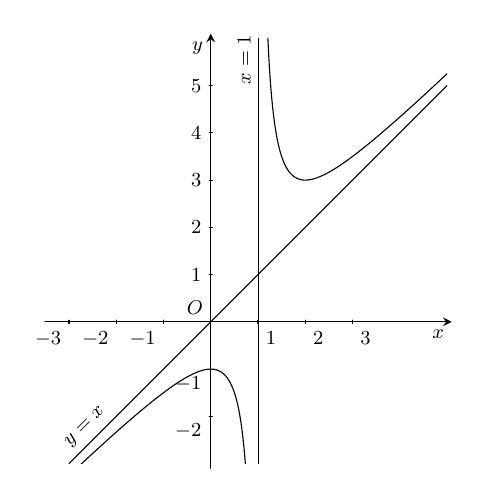
\begin{tikzpicture}[scale=0.6,font=\small,line join=round
		,line cap=round,>=stealth]
		\tikzset{every node/.style={scale=0.8}}
		\draw[->] (-3.51,0)--(5.1,0) node[below left] {$x$};
		\draw[->] (0,-3.1)--(0,6.1) node[below left] {$y$};
		\draw (0,0) node [above left] {$O$};
		\foreach \x/\nx in {1/1,2/2,3/3}
		\draw[thin] (\x,1pt)--(\x,-1pt) node [below right] {$\nx$};
		\foreach \x/\nx in {-3/-3,-2/-2,-1/-1}
		\draw[thin] (\x,1pt)--(\x,-1pt) node [below left] {$\nx$};
		\foreach \y/\ny in {-2/-2,-1/-1}
		\draw[thin] (1pt,\y)--(-1pt,\y) node [below left] {$\ny$};
		\foreach \y/\ny in {1/1,2/2,3/3,4/4,5/5}
		\draw[thin] (1pt,\y)--(-1pt,\y) node [left] {$\ny$};
		
		\draw[thin] (1.01,-3)--(1.01,6)node[pos=0.95, sloped, above] {$x=1$};
		\begin{scope}
			\clip (-3.5,-3) rectangle (5,6);
			\draw[samples=200,domain=-5:0.99,smooth,variable=\x] plot (\x,{(1*((\x)^2)+-1*(\x)+1)/(1*(\x)+-1)});
			\draw[samples=200,domain=1.01:7,smooth,variable=\x] plot (\x,{(1*((\x)^2)+-1*(\x)+1)/(1*(\x)+-1)});
		%	\draw[,thin] (-5.1,-7.1)--(7.1,5.1);
		\draw (-3,-3)--(5,5) node[pos=0.07, sloped, above] {$y = x$};
		\end{scope}
		
	\end{tikzpicture}}
	\loigiai{
	Ta thấy đây là đồ thị hàm số phân thức bậc hai trên bậc nhất nên hàm số có dạng\\ $y=\dfrac{ax^2+bx+c}{dx+e}$. \\
	Mặc khác, dựa vào đồ thị, ta thấy $x=1$ là đường tiệm cận đứng của đồ thị hàm số nên mẫu số có dạng $dx+e = x-1.$\\
	Vậy hàm số có dạng
	$$
	y=\dfrac{ax^2+bx+c}{x-1}.
	$$
	Đồ thị có đường thẳng $y=x$ là đường tiệm cận xiên, ta thực hiện phép chia đa thức
	$$\frac{ax^2+bx+c}{x-1}
	= ax + (a+b) + \frac{a+b+c}{x-1}.$$
	Để tiệm cận xiên đúng bằng $y=x$ thì hệ số của $x$ phải bằng $1$ và hằng số phải bằng $0$.\\
	 Do đó: $a = 1$, $a+b = 0 \Rightarrow b = -1.$\\
	 Khi đó hàm số có dạng
	 $$
	 y=\dfrac{x^2-x+c}{x-1}.
	 $$
Từ đồ thị ta thấy đồ thị hàm số đi qua điểm $(0;-1)$. Do đó ta có
$$
-1=\dfrac{0^2-0+c}{0-1}\Leftrightarrow -1=\dfrac{c}{-1}\Rightarrow c=1.
$$
Vậy hàm số cần tìm là $ y=\dfrac{x^2-x+1}{x-1}.$
	}
\end{ex}

%%%==============HetCau_EX12==============%%%
\TNTF
%%%==============Cau_EX1==============%%%
\begin{ex}%[2D1V5-1]%[Lớp 12 - Đề thi GK1 - THPT Ba Điềm - TPHCM]%[Hoàng Anh Tuấn]
	\immini[thm]{Cho hàm số $y=f(x)=ax^3+bx^2+cx+d$ có đồ thị như hình dưới đây
	\choiceTF
	{Hàm số đồng biến trên khoảng $(-1;+\infty)$}
	{Hàm số đạt cực tiểu tại $x=1$}
	{\True Đồ thị hàm số cắt $Oy$ tại điểm có toạ độ $(0;1)$}
	{\True Trong 4 số $a$, $b$, $c$, $d$ có $3$ số dương}
	}{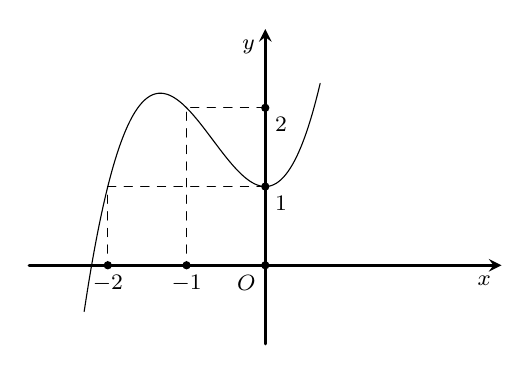
\begin{tikzpicture}[line join = round, line cap=round,>=stealth,font=\footnotesize,scale=1,samples=200]
			
			\def \xtrai{-3} \def\xphai{3}
			\draw[->,line width=1pt] (\xtrai,0)--(\xphai,0) coordinate (x) node[below left]{$x$};	
			\def \yduoi{-1} \def\ytren{3}
			
			\draw[->,line width=1pt] (0,\yduoi)--(0,\ytren)coordinate (y) node[below left]{$y$};			
			
			draw[opacity=0.1] (\xtrai,\yduoi) grid (\xphai,\ytren);
			\fill (0,0) coordinate (O) circle(1.5pt) node[below left]{$O$};
			\draw plot[domain=-2.3:0.7] (\x,{(\x)^3+2*(\x)^2+1})
			;
			\draw[dashed] 
			(0,2)--(-1,2) -- (-1,0)
			(0,1)--(-2,1) -- (-2,0)
			;
			\foreach	\x	in	{-2,-1}
			\fill (\x,0) circle(1.5pt) node[below]{$\x$}
			;
			\foreach	\y	in	{1,2}
			\fill (0,\y) circle(1.5pt) node[below right]{$\y$}
			;
		\end{tikzpicture}}
	\loigiai{
		\begin{itemchoice}
			\itemch \textbf{Sai}.\\
			Từ đồ thị hàm số, ta thấy trên khoảng $(-1;+\infty)$ hàm số không đồng biến.
			\itemch \textbf{Sai}.\\
			Từ đồ thị hàm số, ta thấy hàm số đạt cực tiểu tại $x=0$.
			\itemch \textbf{Đúng}.\\
			Dựa vào đồ thị hàm số $f(x)$, ta thấy hàm số cắt trục $Oy$ tại điểm $(0;1)$.
			\itemch \textbf{Đúng}.\\
			Đồ thị hàm số đi qua điểm $(0;1)$ nên ta có $f(0)=a\cdot 0^3+b\cdot 0^2+c\cdot 0+d=1\Rightarrow d=1$.\\
			Đồ thị hàm số đi qua điểm $(-1;2)$ nên ta có $$f(-1)=a\cdot (-1)^3+b\cdot (-1)^3+c\cdot (-1)+d=2\Rightarrow -a+b-c+d=2.$$
			Đồ thị hàm số đi qua điểm $(-2;1)$ nên ta có $$f(-2)=a\cdot (-2)^3+b\cdot (-2)^3+c\cdot (-2)+d=1\Rightarrow -8a+4b-2c+d=1.$$
			Từ $y=ax^3+bx^2+cx+d\Rightarrow y'=3ax^2+2bx+c$.\\
			 Mặt khác, hàm số đạt cực tiểu tại $x=0$ nên $0=3\cdot 0^2\cdot a+2\cdot 0.b+c\Rightarrow c=0$. \\
			Do đó ta có hệ $\heva{&-a+b-c+1=2\\&-8a+4b-2c+1=1\\&c=0\\&d=1}\Rightarrow \heva{a=1\\b=2\\c=0\\d=1.}$\\
			Vậy trong 4 số $a$, $b$, $c$, $d$ có ba số dương.\\
			\end{itemchoice}
	}
\end{ex}

%%%==============HetCau_EX1==============%%%


%%%==============Cau_EX2==============%%%

\begin{ex}%[2D1H4-1]%[Lớp 12 - Đề thi GK1 - THPT Ba Điềm - TPHCM]%[Hoàng Anh Tuấn]
Cho hàm số $f(x)=\dfrac{2x-3}{x^2+4}$.
	\choiceTF
	{\True Hàm số $f(x)$ có điểm cực đại là $x=4$}
	{\True Đồ thị hàm số $y=f(x)$ nhận trục hoành làm tiệm cận ngang}
	{\True $f(24)=\dfrac{9}{116}$ }
	{Tập giá trị của hàm số đã cho là đoạn $[a;b]$ thì $3a+4b=2$}
	\loigiai{
		\begin{itemchoice}
			\itemch \textbf{Đúng}.\\
			Từ $f(x)=\dfrac{2x-3}{x^2+4}\Rightarrow f'(x)=\dfrac{2(x^2+4)-2x(2x-3)}{(x^2+4)^2}=\dfrac{-2x^2+6x+8}{(x^2+4)^2}$.\\
			$f'(x)=0\Leftrightarrow \dfrac{-2x^2+6x+8}{(x^2+4)^2}=0$. \\
			Suy ra $-2x^2+6x+8=0\Leftrightarrow \hoac{&x=4\\&x=-1.}$\\
			Ta có bảng biến thiên: 
				\begin{center}
				
\begin{tikzpicture}
					\tkzTabInit[nocadre=false,espcl=2.5,lgt=1.5,deltacl=0.6]
					{$x$/0.7,$f'(x)$/0.7,$f(x)$/2.1}
					{$-\infty$,$-1$,$4$,$+\infty$}
					\tkzTabLine{,-,0,+,0,-,}
					\tkzTabVar{+/$0$,-/$-1$,+/$\dfrac{1}{4}$,-/$0$}
				\end{tikzpicture}
			\end{center}
			Từ bảng biến thiên ta thấy hàm số $f(x)$ có điểm cực đại là $x=4$
			\itemch \textbf{Đúng}.\\
			Ta có: $\lim\limits_{x\to +\infty}f(x)=\lim\limits_{x\to +\infty}\dfrac{2x-3}{x^2+4}=0;\lim\limits_{x\to -\infty}f(x)=\lim\limits_{x\to -\infty}\dfrac{2x-3}{x^2+4}=0$.\\
			 Do đó, đồ thị hàm số có đường tiệm cận ngang là $y=0$. 
			\itemch \textbf{Đúng}.\\
			$f(24)=\dfrac{2\cdot 24-3}{24^2+4}=\dfrac{45}{580}=\dfrac{9}{116}$.
			\itemch \textbf{Sai}.\\
			Từ bảng biến thiên, ta thấy tập giá trị của hàm số $f(x)$ là đoạn $\left[-1;\dfrac{1}{4}\right]$.\\
			 Do đó $a=-1;b=\dfrac{1}{4}$.\\
			  Suy ra $3a+4b=3\cdot (-1)+4\cdot \dfrac{1}{4}=-2.$ 
		\end{itemchoice}
	}
\end{ex}

%%%==============HetCau_EX2==============%%%

%%%==============Cau_EX3==============%%%
\begin{ex}%[2D1V2-1]%[Lớp 12 - Đề thi GK1 - THPT Ba Điềm - TPHCM]%[Hoàng Anh Tuấn]
	Cho hàm số $f(x)=\log_{\frac{1}{2}}(x^2-5x+4).$
	\choiceTF
	{Hàm số $y=f(x)$ đồng biến trên khoảng $\left(-\infty;\dfrac{5}{2}\right)$}
	{\True Hàm số $y=f(x)$ có đạo hàm $f'(x)=\dfrac{5-2x}{(x^2-5x+4)\ln 2}$}
	{Hàm số $y=f(x)$ có tập xác định $\mathscr{D}=(-\infty;1]\cup [4;+\infty)$}
	{Hàm số có một điểm cực trị}	
	\loigiai{
	\begin{itemchoice}
		\itemch \textbf{Sai}.\\
		Hàm số $f(x)=\log_{\frac{1}{2}}(x^2-5x+4)$ xác định khi $x^2-5x+4>0\Rightarrow\hoac{x>4\\x<1.}$\\
		Suy ra tập xác định của hàm số là $\mathscr{D}=(-\infty;1)\cup (4;+\infty)$.\\
		 Do đó hàm số không xác định trên $\left(-\infty;\dfrac{5}{2}\right)$ nên không đồng biến trên khoảng $\left(-\infty;\dfrac{5}{2}\right)$.
		\itemch \textbf{Đúng}.\\
		$f(x)=\log_{\frac{1}{2}}(x^2-5x+4)\Rightarrow f'(x)=\dfrac{(x^2-5x+4)'}{(x^2-5x+4)\cdot \ln\dfrac{1}{2}}=\dfrac{5-2x}{(x^2-5x+4)\cdot \ln2}$.
		\itemch \textbf{Sai}.\\
		Ta có tập xác định của hàm số $y=f(x)$ là $\mathscr{D}=(-\infty;1)\cup (4;+\infty)$.
		\itemch \textbf{Sai}.\\
		Ta có $\dfrac{5-2x}{(x^2-5x+4)}\cdot \ln2=0\Rightarrow x=\dfrac{5}{2}$.\\
		 Vì $1<\dfrac{5}{2}<4$ nên $x=\dfrac{5}{2}$ không thuộc$\mathscr{D}$.\\ 
		 Do đó hàm số không đạt cực trị tại $x=\dfrac{5}{2}$.
	\end{itemchoice}
	}
\end{ex}
%%%==============HetCau_EX3==============%%%

%%%==============Cau_EX4==============%%%
\begin{ex}%[2D1V5-8]%[Lớp 12 - Đề thi GK1 - THPT Ba Điềm - TPHCM]%[Hoàng Anh Tuấn]
	Một chất điểm chuyển động theo phương trình $s(t) = -t^3 + 9t^2 + 21t + 9$ với $t$ tính bằng giây (s) là khoảng thời gian tính từ lúc vật bắt đầu chuyển động và $s$ tính bằng mét (m) là quãng đường vật đi được trong thời gian đó.
	\choiceTF
	{\True Vận tốc của chất điểm tại giây thứ 2 là $45$ m/s}
	{\True Vận tốc của chất điểm chuyển động tại thời điểm $t$ (giây) là $v(t) = -3t^2 + 18t + 21$}
	{Quãng đường chất điểm đi được từ lúc bắt đầu đến lúc dừng hẳn là $255$ m}
	{\True Vận tốc chuyển động của chất điểm đạt giá trị lớn nhất tại thời điểm $t=3$ s}	
	\loigiai{
		\begin{itemchoice}
			\itemch \textbf{Đúng}.\\
			Vận tốc của chất điểm tại thời điểm $t$ được tính bằng đạo hàm của quãng đường theo thời gian.\\
			 Suy ra
			$v(t)=s'(t)=-3t^2+18t+21$.\\
			 Vận tốc của chất điểm tại giây thứ 2 là $v(2)=-3\cdot 2^2+18\cdot 2+21=45$.
			\itemch \textbf{Đúng}.\\
			Vận tốc của chất điểm tại thời điểm $t$ được tính bằng đạo hàm của quãng đường theo thời gian. Suy ra
			$v(t)=s'(t)=-3t^2+18t+21$.
			\itemch \textbf{Sai}.\\
			Thời điểm vật dừng lại hẳn là nghiệm của phương trình
			$$-3t^2+18t+21=0\Leftrightarrow (t-7)(t+1)=0\Leftrightarrow \hoac{&t=7\\&t=-1 \text{ (loại) } }$$
			Vậy thời gian vật dừng hẳn là $t=7$.\\
			Quãng đường chất điểm đi được từ lúc bắt đầu ($t=0$) đến lúc dừng hẳn ($t=7$) là\\
			$$s(7)-s(0)=(-7^3+9\cdot 7^2+21\cdot 7+9)-(-0^3+9\cdot 0^2+21\cdot 0+9)=254-9=245 \text{ (m)}.$$ 
			\itemch \textbf{Đúng}.\\
			Từ $v(t)=-3t^2+18t+21\Rightarrow v'(t)=-6t+18$.\\
			$v'(t)=0\Leftrightarrow -6t^2+18=0\Rightarrow t=3$. Ta có bảng biến thiên
				\begin{center}
				
\begin{tikzpicture}
					\tkzTabInit[nocadre=false,espcl=2.5,lgt=1.5,deltacl=0.6]
					{$t$/0.7,$v'(t)$/0.7,$v(t)$/2.1}
					{$0$,$3$,$+\infty$}
					\tkzTabLine{,-,0,+,}
					\tkzTabVar{-/$21$,+/$48$,-/$-\infty$}
				\end{tikzpicture}
			\end{center}
			Vậy vận tốc lớn nhất của chất điểm đạt được là $48$ m/s và đạt được khi $t=3$.
		\end{itemchoice}
	}
\end{ex}
%%%==============HetCau_EX1==============%%%
\TNSA
\begin{ex}%[2D1V3-6]%[Dự án A đợt 1 năm học 2025-2026, BCTuan]
	\immini[thm]{
		Một trang sách có dạng hình chữ nhật với diện tích là $600$ cm$^2$. Sau khi để lề trên và lề dưới đều là $2$ cm, lề trái là $3$ cm và lề phải là $2$ cm. Tính diện tích lớn nhất của phần chữ in vào cuốn sách (kết quả làm tròn đến hàng đơn vị).
	}{
		\begin{tikzpicture}[>=stealth,smooth,line join=round,line cap=round,font=\footnotesize,scale=1]
			\path
			(0,0) coordinate (B)
			(0:3) coordinate (A)
			(90:4) coordinate (C)
			($(C)-(B)+(A)$) coordinate (D)
			;
			\fill[blue!20] (0.3,0.35) rectangle (2.7,3.65);
			\draw[dashed] (0.3,0.35) rectangle (2.7,3.65);
			;
			\draw (A)--(B)--(C)--(D)--(A)
			;
		\end{tikzpicture}
	}
	\shortans{$401$}
	\loigiai{
		Gọi chiều dài của trang giấy là $x$; chiều rộng của trang giấy là $\dfrac{600}{x}$.\\
		Chiều dài phần chữ in là $x-4$; chiều rộng phần chữ in là $\dfrac{600}{x}-5$.\\
		Từ đó điều kiện của $x$ là $4<x<120$.\\
		Diện tích phần chữ in là $(x-4)\left(\dfrac{600}{x}-5\right)=-5x-\dfrac{2\,400}{x}+620$.\\
		Xét hàm số $f(x)=-5x-\dfrac{2\,400}{x}+620$ trên $(4;120)$. Ta có
		$$
		f'(x)=-5+\dfrac{2\,400}{x^2}; f'(x)=0 \Leftrightarrow\hoac{&x=4\sqrt{30}\\&x=-4\sqrt{30}\notin(0;120).}
		$$
		Bảng biến thiên
		\begin{center}
			\begin{tikzpicture}[font=\normalsize,t style/.style={style=solid}]
				\tkzTabInit[nocadre=false, lgt=1.2, espcl=2.5, deltacl=0.5]
				{$x$/0.75, $f'(x)$/0.75, $f(x)$/3}
				{$0$, $4\sqrt{30}$, $+\infty$}
				\tkzTabLine{ , +, 0, -}
				\path
				($(N13)!0.1!(N12)$) node (A1){$-\infty$}
				($(N23)!0.8!(N22)$) node (A2){$f\left(4\sqrt{30}\right)$}
				($(N33)!0.1!(N32)$) node (A3){$+\infty$};
				\foreach \x/\y in {A1/A2, A2/A3}{
					\draw[-stealth] (\x)--(\y);
				}
			\end{tikzpicture}
		\end{center}
		Dựa vào bảng biến thiên ta có diện tích phần chữ in lớn nhất là $f\left(4\sqrt{30}\right)\approx 401$ (cm$^2$).
	}
\end{ex}
%-----Câu 1
\begin{ex}%[2D1H2-1]%[Dự án A đợt 1 năm học 2025-2026, BCTuan]
	Hàm số $y=\dfrac{x^2-x+1}{x-1}$ có giá trị cực đại và giá trị cực tiểu lần lượt là $a$ và $b$. Tính $3a+2b$.
	\shortans{$3$}
	\loigiai{
		Ta có $y'=\dfrac{x^2-2x}{(x-1)^2}$, $\forall x\ne 1$,
		$y'=0\Leftrightarrow \hoac{&x=0\\&x=2.}$\\
		Bảng biến thiên
		\begin{center}
			
\begin{tikzpicture}
				\tkzTabInit[nocadre=false,lgt=1.2,espcl=2.5,deltacl=0.6]
				{$x$ /0.8,$y'$ /0.8,$y$ /2.3}
				{$-\infty$,$0$,$1$,$2$,$+\infty$}
				\tkzTabLine{,+,$0$,-,d,-,$0$,+,}
				\tkzTabVar{-/$-\infty$,+/$-1$,-D+/$-\infty$/$+\infty$,-/$3$,+/$+\infty$}
			\end{tikzpicture}
		\end{center}
		Dựa vào bảng biến thiên ta có giá trị cực đại của hàm số là $a=-1$ và giá trị cực tiểu của hàm số là $b=3$.\\
		Vậy $2a+3b=3$.
	}
\end{ex}
\begin{ex}%[2D1H2-2]%[Dự án A đợt 1 năm học 2025-2026, BCTuan]
	\immini[thm]{
		Cho hàm số $y=ax^3+bx^2+cx+d$ có đồ thị như hình vẽ bên. Giá trị $S=a+b$ bằng
	}
	{
		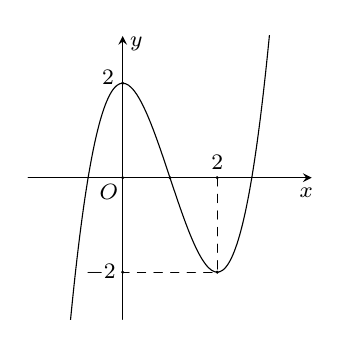
\begin{tikzpicture}[font=\footnotesize,line join=round, line cap=round, >=stealth,scale=0.6] 
			\def \xmin{-2}\def \xmax{4}\def \ymin{-3}\def \ymax{3} 
			\draw[->] (\xmin,0)--(\xmax,0) node[shift=(-110:0.2)] {$x$};
			\draw[->] (0,\ymin)--(0,\ymax) node[shift=(-30:0.2)] {$y$};
			\fill (0,0) circle(1pt) node[shift=(-135:0.25)]{$O$}
			(1,0) circle(1pt)
			(2,0) circle(1pt) node[shift=(90:0.2)]{$2$}
			(0,-2) circle(1pt) node[shift=(180:0.28)]{$-2$}
			(0,2) circle(1pt) node[shift=(160:0.2)]{$2$}
			(2,-2) circle(1pt);
			\draw[dashed] (2,0)|-(0,-2);
			\clip (\xmin,\ymin) rectangle (\xmax,\ymax);
			\draw[smooth,samples=100,domain=\xmin:\xmax] plot(\x, {(\x)^3-3*(\x)^2+2});
		\end{tikzpicture}		
	}
	\shortans{$-2$}
	\loigiai{Đặt $f(x)=ax^3+bx^2+cx+d$.
		Ta có $f'(x)=3ax^2+2bx+c$.\\
		Đồ thị hàm số $(C)$ có $2$ điểm cực trị là $(0;2)$ và $(2;-2)$ nên ta có hệ phương trình
		\[\heva{&f(0)=2\\
			&f(2)=-2\\
			&f'(0)=0\\
			&f'(2)=0} \Leftrightarrow \heva{& 
			d=2\\
			&8a+4b+2c+d=-2\\
			&c=0\\
			&12a+4b+c=0} \Leftrightarrow \heva{&
			a=1 \\
			&b=-3 \\
			&c=0 \\
			&d=2.}\]
		Vậy hàm số là $f(x)=x^3-3x^2+2$.\\
		Khi đó $a=1$, $b=-3$ nên $a+b=-2$.
	}
\end{ex}
\begin{ex}%[2D1H5-1]%[Dự án A đợt 1 năm học 2025-2026, BCTuan]
	Cho hàm số $f(x)=\dfrac{ax+b}{2x+d}$ ($a$, $b$, $d \in \mathbb{R}$). Biết rằng đồ thị hàm số đã cho đi qua điểm $(-1;7)$ và giao điểm hai tiệm cận là $(-2;3)$. Giá trị biểu thức $\dfrac{2a+3b+d+8}{14}$ bằng
	\shortans{6}
	\loigiai{
		Vì giao điểm của hai đường tiệm cận là $(-2;3)$ nên đồ thị hàm số có $2$ đường tiệm cận là $x=-2$ và $y=3$.\\
		Từ đó ta có $-\dfrac{d}{2}=-2\Leftrightarrow d=4$.\\
		Và $\dfrac{a}{2}=3\Leftrightarrow a=6$.\\
		Đồ thị hàm số đi qua điểm $(-1;7)$ nên $7=\dfrac{-a+b}{-2+d}\Leftrightarrow b=20$.\\
		Vậy $\dfrac{2a+3b+d+8}{14}=\dfrac{2\cdot 6+3\cdot 20+4+8}{14}=6$.
	}	
\end{ex}
\begin{ex}%[2D1V3-6]%[Dự án A đợt 1 năm học 2025-2026, BCTuan]
	Một trang trại rau sạch ở Đà Lạt mỗi ngày thu hoạch được $1$ tấn rau. Mỗi ngày, nếu giá bán rau là $30$ nghìn đồng$/\mathrm{kg}$ thì bán hết rau, nếu giá bán rau tăng $1$ nghìn đồng$/\mathrm{kg}$ thì số rau thừa tăng $20$ kg. Số rau thừa này được thu mua hết để làm thức ăn chăn nuôi với giá $2$ nghìn đồng$/\mathrm{kg}$. Hỏi để mỗi ngày thu được số tiền bán rau lớn nhất thì trang trại đó nên bán rau với giá bao nhiêu nghìn đồng?
	\shortans[oly]{$41$}
	\loigiai{
		Gọi $x$ (nghìn đồng) là giá bán rau sau khi tăng giá ($x\ge 30$).\\
		Vì tăng giá $1$ nghìn đồng thì thừa $20$ kg rau nên số kg rau thừa là $20(x-30)=20x-600$ kg.\\
		Số kg rau được bán là $1\,000-(20x-600)=1\,600-20x$ kg.\\
		Số tiền thu được từ bán rau là $$f(x)=(1\,600-20x)x+(20x-600)\cdot2=-20x^2+1\,640x-1\,200 \ (\text{nghìn đồng}).$$
		Ta có $f'(x)=-40x+1\,640$; $f'(x)=0\Leftrightarrow x=41$.\\
		Bảng biến thiên
		\begin{center}
			
\begin{tikzpicture}
				\tkzTabInit[espcl=2.5,lgt=1.5]
				{$x$/0.7,$f'(x)$/0.7,$f(x)$/2.2}
				{$30$,$41$,$+\infty$}
				\tkzTabLine{,+,0,-,}
				\tkzTabVar{-/$ $,+/$ $,-/$ $}
			\end{tikzpicture}
		\end{center}
		Vậy nên bán rau với giá $41$ nghìn đồng.
	}
\end{ex}
\begin{ex}%[2D1V5-8]%[Dự án A đợt 1 năm học 2025-2026, BCTuan]
	Thầy Hiếu tham dự giải \lq\lq Đi bộ trực tuyến Ngành Giáo dục và Đào tạo Edu Run-HCMC\rq\rq\ năm 2025. Quãng đường thầy Hiếu đi được biểu diễn bằng hàm số $s(t)=at^3+bt^2+ct+d$ (với $a\ne 0$) có đồ thị như hình vẽ (trong đó $t$ là thời gian tính bằng giờ, $s$ là quãng đường tính bằng km). Khi đó, vận tốc tối đa của thầy Hiếu đạt được trong quá trình đi bộ là bao nhiêu (đơn vị km/h)?
	\begin{center}
		\begin{tikzpicture}[yscale=0.2,scale=.7, font=\footnotesize, line join=round, line cap=round,>=stealth]
			\def\a{2} \def\b{-1} \def\c{1} \def\d{-1} 
			\def\xmin{-1} \def\xmax{7}
			\def\ymin{-5} \def\ymax{28}
			\draw[->] (\xmin,0)--(\xmax,0) node [below]{$t$\,(h)};
			\draw[->] (0,\ymin)--(0,\ymax) node [left]{$s$\,(km)};
			\node at (0,0) [below left]{$O$};
			\foreach \x in {1,2,3,4,5,6}{\draw [fill = red] (\x,0) circle(1pt) node[below]{$\x$};};
			\foreach \x in {6,12,18,24}{\fill (0,\x) circle(1pt) node[left]{$\x$};};
			\clip (\xmin+0.1,\ymin+0.1) rectangle (\xmax-1.1,\ymax-0.1);
			\draw[smooth,samples=300,domain=(0:\xmax)] plot(\x,{-0.75*(\x)^3+4.5*(\x)^2});
			\draw[dashed] (2,0)--(2,12)--(0,12) (4,0)--(4,24)--(0,24);
		\end{tikzpicture} 
	\end{center}
	\par
	\shortans{9}
	\loigiai{
		Dựa vào đồ thị ta thấy đồ thị hàm số đi qua các điểm: $O(0;0)$, $A(2;12)$, $B(4;24)$ và nhận $B(4;24)$ làm một điểm cực trị.\\
		Ta có $s(t)=at^3+bt^2+ct+d\Rightarrow s'(t)=3at^2+2bt+c$.\\
		Khi đó ta có hệ sau $\heva{
			& s(0)=0 \\
			& s(2)=12 \\
			& s(4)=24 \\
			& {s}'(4)=0}
		\Leftrightarrow \heva{
			& d=0 \\
			& 8a+4b+2c+d=12 \\
			& 64a+16b+4c+d=24 \\
			& 48a+8b+c=0}
		\Leftrightarrow \heva{
			& a=-\dfrac{3}{4} \\
			& b=\dfrac{9}{2} \\
			& c=0 \\
			& d=0.}$\\
		Nên $s(t)=-\dfrac{3}{4}{t^3}+\dfrac{9}{2}{t^2}\Rightarrow v(t)=s'(t)=-\dfrac{9}{4}{t^2}+9t$.\\
		Thầy Hiếu dừng đi bộ khi $v(t)=0\Leftrightarrow -\dfrac{9}{4}{t^2}+9t=0
		\Leftrightarrow \heva{&t=0\\& t=4.}$\\
		Bài toán trở thành tìm giá trị lớn nhất của $v(t)$ trên $[0;4]$.\\
		Ta có $v'(t)=-\dfrac{9}{2}t+9\Rightarrow v'(t)=0\Leftrightarrow t=2$.\\
		Khi đó $v(0)=0$, $v(2)=9$, $v(4)=0$.\\
		Vậy vận tốc lớn nhất mà thầy Hiếu đạt được là $9$\,(km/h) tại thời điểm $t=2$\,(h).}
\end{ex}
\Closesolutionfile{ans}

